\documentclass[12pt,letterpaper]{article}
\usepackage{fullpage}
\usepackage[top=2cm, bottom=4.5cm, left=2.3cm, right=2.3cm]{geometry}
\usepackage{amsmath,amsthm,amsfonts,amssymb,amscd}
\usepackage{lastpage}
\usepackage{enumerate}
\usepackage{fancyhdr}
\usepackage{mathrsfs}
\usepackage{xcolor}
\usepackage{graphicx}
\usepackage{listings}
\usepackage{hyperref}

\hypersetup{%
  colorlinks=true,
  linkcolor=blue,
  linkbordercolor={0 0 1}
}
\usepackage{wrapfig}
\renewcommand\lstlistingname{Algorithm}
\renewcommand\lstlistlistingname{Algorithms}
\def\lstlistingautorefname{Alg.}

\lstdefinestyle{Python}{
    language        = Python,
    frame           = lines, 
    basicstyle      = \footnotesize
}

\setlength{\parindent}{0.0in}
\setlength{\parskip}{0.05in}

% Edit these as appropriate
\newcommand\course{CS 639}

%\pagestyle{fancyplain}
\headheight 35pt
\usepackage{xcolor}
% hyperref link defaults to "blue" (0000ff) as this matches our publisher produced pdf style
\definecolor{xlinkcolor}{cmyk}{1,1,0,0}
\usepackage{hyperref}
\fancypagestyle{firstpage}{
  \chead{\textbf{\Large  Bayesian vs Frequentist Approach \\in Medical Research \\}}
  \rhead{\course \\ \today}
  \lhead{ Harsh Sahu \\Lekshmi Thulasidharan}
  \lfoot{}
  \cfoot{}
  \rfoot{\small\thepage}
  \headsep 3em
}


\usepackage{amsmath}
\PassOptionsToPackage{hyphens}{url}
\fancypagestyle{normal}{
  %\renewcommand{\headrulewidth}{0.5pt}
  \headsep 3em
}

% Set the default page style to 'normal'
%\pagestyle{headings}
%\headsep 2em
%\fancyhead[R]{\rightmark}
%\renewcommand{\subsectionmark}[1]{\markright{#1}}

\pagestyle{headings}
\headsep 2em

%% In response to request from AAS 

\begin{document}
\par
%\thispagestyle{fancy}
\thispagestyle{firstpage}
\section{Introduction}
In medical research, statistical methods are commonly used to analyze data and draw conclusions. Two common approaches are the Bayesian and frequentist approaches. In simple words, Bayesian statistics involves the use of past/existing knowledge (a.k.a prior) along with the new data to make predictions, while frequentist statistics involves making inferences based on the observed data alone. We start this review with a short overview of each approach followed by the application of Bayesian and frequentist methods in predicting the risk of dementia in older adults. We then attempt to do a comparison study.

%Specifically, we try to answer the following questions:
%\begin{itemize}
%   \item What are the relative strengths and weaknesses of Bayesian and frequentist methods in the context of medical research?
%    \item  Under which circumstances do the two approaches lead to similar or different conclusions?
%    \item Does the use of one of these approaches increase the potential for breakthroughs in medical research compared to the other?
%    \item What are the drawbacks of each approach?
%\end{itemize}

\subsection{Frequentist Approach}

The frequentist approach \cite{chen2018,mary} is a widely used statistical approach for making predictions. It considers probability of an event as the frequency of an event occurring in a large sample of data or repeated sampling of the same experiment. So it makes predictions based only on the data at hand. The basic idea is to evaluate the parameters of interest of the data which is not known. If we have a large sample of data, then we can choose the most likely value of the parameter which generates a similar data. This method is also called the Maximum Likelihood parameter estimation (MLE). Mathematically, the probability of observing the data (say $X$) given a set of parameters (say $\theta$) can be denoted by the likelihood function $\mathcal{L}(X|\theta)$. Then what we are looking for is essentially $\hat{\theta}=argmax_\theta [\mathcal{L}(X|\theta)]$. Some statistical analysis techniques that comes under the frequentist approach are linear regression, logistic regression etc. In both of these methods, the parameters in the model(linear model for linear regression and a sigmoid function for logistic regression) are estimated using MLE or in other words the residuals between the actual response variable of the data and the predicted response variable from the model is minimized. 

% A part of this review is dedicated to the application of frequentist approach in medical research which has been once the most commonly used method for clinical data analysis due its simple and straightforward nature.  

\subsection{Bayesian Approach}
Bayesian approach \cite{Croat,abc} is another statistical approach, based on Bayes's theorem to make predictions. In contrast to frequentist approach, the probability of an event also depends on the pre-existing knowledge about the data (called prior) instead of the data alone. This prior is then combined with current experiment data to make a conclusion on the test. While Frequentist statistics tries to estimate $\mathbb{P}( x | \theta)$, Bayesian statistics estimates $\mathbb{P}( \theta | x)$. It makes prior assumptions about the distribution of $\theta$ and assumes some $\mathbb{P}(\theta)$. It then estimates the posterior probability as $ \mathbb{P}( \theta | x) \propto \mathbb{P}( x | \theta) \mathbb{P}(\theta)$. That is in the Bayesian approach, the parameters that we are trying to estimate are treated as random variables, whereas in frequentist approach they are fixed.\\

Here, we review and compare two papers which tries to identify the risk factors for Dementia. The first paper \textit{Predicting risk of dementia in older adults} \cite{barnes2009} uses a frequentist approach whereas the second paper \textit{Bayesian Approach to identifying potential risk factors for dementia} \cite{Wen} uses the bayesian approach to predict the risk of dementia.


%\subsection{Comparison}
%Also talk about medical research application. Case study : Dementia
% \newpage
\section{Application of frequentist approach in risk prediction of dementia in older adults}
Dementia \cite{dem} is a common yet severe condition that primarily affects elder population. This is an umbrella term for conditions which could impair a person's ability to perform day to day activities since it has a detrimental effect on their cognition. For example, those who have dementia will experience memory loss, difficulty with communication and reasoning along with changes in psychological health. Unfortunately, there is currently no known cure for dementia. For this reason, it is extremely important to identify the individuals who are at very high risk for dementia early on, since this allows for incorporating lifestyle changes and treatments which could potentially slow the rate of progression of this condition. A straightforward method which allows the early identification of risk factors of dementia is by utilising statistical techniques to generate a risk score model. Researchers assign a score to every possible risk factors including demographic factors that could contribute to the development of dementia. Once we have the model, we can screen people and classify them into low, moderate and high risk populations.\\

Within the frequentist approach, one statistical technique that can be highly effective in creating risk prediction models is the ``Logistic regression''. In this section, we review Barnes et al. (2009) \cite{barnes2009}, where they developed one such risk score model i.e., a late life dementia index which can be used to accurately predict the chances of a person developing dementia in 6 years based on several risk factors using Logistic Regression. The tool they developed can be used to classify individuals into low, moderate and high risk categories for dementia, and hence serves as an excellent aid for monitoring vulnerable adults for dementia symptoms to start their treatment early on.  

\subsection{Logistic Regression}

Logistic Regression is a useful method for classification problems where we want to find the probability of a variable belongs to a particular category \cite{intro2013}. So, this analysis is best for predicting binary outcomes like yes or no. In medical research this could translate into the probability of a patient developing a disease given one or more input variables (which would be the suspected risk factors). The probability is modelled using a logistic function which is a sigmoid (Fig.\ref{dvdr}). The function takes a linear combination of the input variables and  and returns an output between 0 and 1. \\

When we have multiple input variables as in the case of risk prediction of a disease, the logistic function takes the form:
\begin{equation}
p(X) =Pr (Y|X)= \frac{e^{\beta_0+\beta_1X_1+\beta_2X_2+...+\beta_pX_p}}{1+e^{\beta_0+\beta_1X_1+\beta_2X_2+...+\beta_pX_p}}
\end{equation}

\begin{wrapfigure}{r}{7cm}
\vspace{-4 mm}
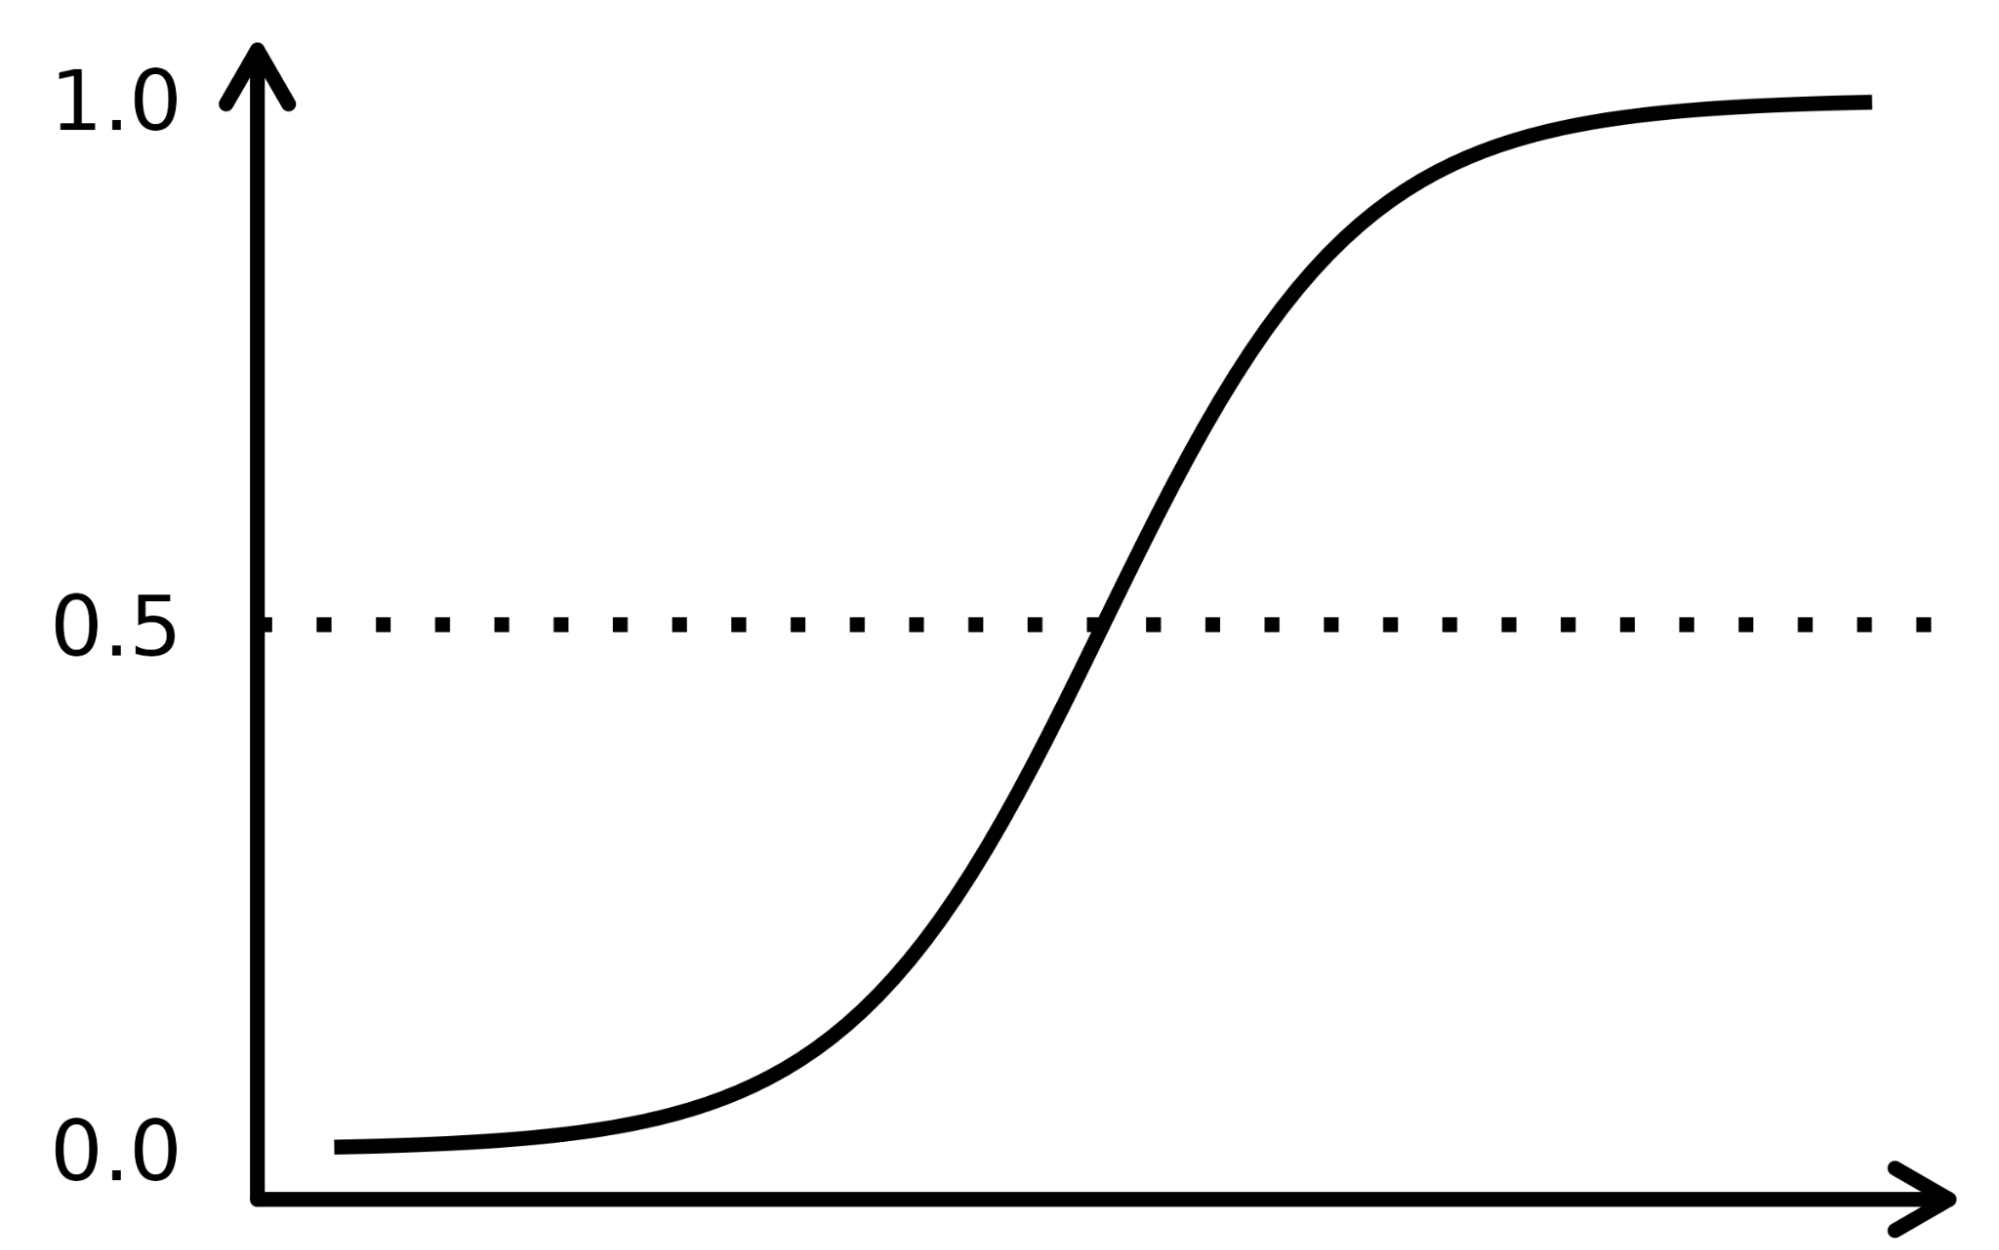
\includegraphics[width=7 cm]{sigmoid.png}
\caption{The sigmoid function curve\cite{sigmoid}}
\label{dvdr}
\end{wrapfigure}
In the context of the paper we are discussing here, $Pr (Y|X)$ would the probability of a person developing dementia (modelled with variable $Y$) given certain risk factors (or predictors) assumed to be independent with each other($X=(X_1,X_2,\dots,X_p)$). The $\beta$ coefficients represent the parameters of the model, with $\beta_0$ being the intercept and $\beta_1,\beta_2,\dots,\beta_p$ being the coefficients for each of the independent variables. The coefficients can be estimated by maximizing the corresponding likelihood function.  

\subsection{Predictors of Dementia}

The data for different predictors were collected from the Cardiovascular Health Cognition Study which was started in 1989–1990 and updated during 1992–1993 \cite{Kuller2003,Lopez2003}. For this study, since the authors are interested in predicting the risk of dementia, they identified the individuals who developed dementia after the data collection as well as those who developed mild cognitive impairment or MCI (this is not as severe as dementia) any time during the follow up period that lasted until 1998-1999 resulting in a sample size of 3,375. 

The authors consider a wide range of predictors for this study and they broadly belong to several categories described below:

(i) Demographic factors - This will help us understand if the risk of developing dementia is related to a person's age, gender, race, ethnicity, income etc.\\
(ii) Pre-exisitng medical conditions: Some of the medical conditions such as a history of stroke, diabetes etc. are known to increase the chances of a person developing dementia. \\
(iii)  Cognitive function : Cognitive function include a person's ability to learn, remember, reason, pay attention etc.  Since dementia is associated with a deterioration of cognitive abilities, this is a very important predictor of this condition. \\
(iv) Physical function measures: This is related to one's ability to perform normal day to day activities without anyone's help. Since dementia is associated with weakened muscle strength and poor coordination, this is a very important risk factor.  \\            
(v) Physical performance measures: Some of the early symptoms of dementia involve taking more than usual time to perform certain normal activities.\\
(vi) Lifestyle factors: Information about one's alcohol consumption rate, smoking habits etc., which are indicators of how healthy a person is. \\
(vii) Psychosocial factors: This takes into consideration, a person's emotional and mental well-being. \\
(viii) Cerebral MRI variables: Includes the presence of small or large tumors, white matter disease (damage to white matter of the brain ) etc. that could seriously affect a person's coordination.\\
(ix) Carotid artery ultrasound variables and Electrocardiogram measurements: Considering this could possibly unveil any correlation of dementia with one's cardiovascular health.\\
(x) Genetic factors: Such as APOE polymorphic alleles in the genes makes a person at the risk of dementia.\\
(xi) Serum measures: Certain blood tests could help understand the underlying condition that causes change in a person's ability to think, reason and remember. \\

This is in fact a lot of predictors. But not all of them will contribute to dementia equally. Some of them could be very good indicators whereas some won't have any effect at all. So before using Logistic Regression to evaluate the finalized logistic coefficients to develop a late life dementia risk score, it makes sense to eliminate some of these predictors from the analysis based on their statistical significance. To do this, careful and rigorous statistical analysis techniques should be used. In the next section, we will look into the methodology followed by the authors to choose the subset of relevant predictors.

\subsection{Methodology for Statistical Analysis}

Before doing any high level statistics to determine the relationship between predictor variables and the target variable (i.e. dementia) using the data of the former, we should always start simple. That is, first step should be to understand the observed data itself. For the entire sample size, we should start by  looking at the distribution of data for every single predictors. This is as simple as plotting a histogram which tells us about the frequency distribution of the variable under study along with its mean, median, range etc. Doing this will help us identify any outliers in the data and also help us quantify what ``high'' and ``low'' means for every variable. In other words, we can identify the cut off value for every variable above which the value of variable is too high and below which it is too low, which will further aid us in the classification of individuals into different subsets for every predictors. For eg. based on the distribution of age of the sample population used in the paper (refer to Table 1 of \cite{barnes2009}), range is from 65-100 years. A cut off was applied at 74 and 79 to divide the population into three groups- 65-74, 75-79 and 80-100. This is essential because some symptoms which are predictive of dementia could be simply a part of natural process of aging. So dividing the population based on age will help in removing any such biases and improve the accuracy of the analysis.\\

It is very important to categorize the variables before looking at their association with dementia. Doing this will not only make it easy to identify existing patterns but also make the data more interpretable by being able to visualize it better. Categorization is a trivial thing to do when the variable we are considering is qualitative. For eg: Among the predictor variables that comes under demographic factors is the gender. It is essential to categorize individuals into biological male and female populations to study the association with dementia. It may not be so straightforward if the variable in the question is quantitative. For eg: one of the risk factors of dementia is poor physical performance when it comes to normal activities. A person who is under high risk of this disease might takes longer time to button a shirt compared to normal people.  Let's say the data of the time taken by a person to button a shirt consists of numbers ranging from 20 sec to 100 sec. To divide the data into what is normal and what is not, we need to determine the cut off point. Let's say normal time to button a shirt is $\leq45$ sec. In this case, we can simply divide the data into two categories by applying the cut off at $45$ sec. We don't need to consider every data point and this makes it easier to study the associations, if any, with dementia. So, it is crucial to accurately determine the cut off as any errors will have the potential to change the distribution of data of the respective groups and this will affect the accuracy of our risk prediction. When it comes to medical research, for some variables, the standard clinical cut off points are available. For eg: total cholesterol $<200$ mg/dL is considered to be normal \cite{cholest} and anything above this value is said to be high. For those variables which doesn't have such a cut off available, the authors apply the Classification and Regression Tree analysis or CART.\\

CART is a decision tree algorithm \cite{cart1,cart2,cart3,cart4}. In this study this is used to identify the cut points for the variables that best differentiate the output of interest, i.e., dementia or no dementia. They used it for both continuous variables such as blood pressure, age etc. and those which are categorical like alcohol consumption (none, moderate. high). The idea is to divide the data based on ``homegeneity". That is CART algorithm will recursively consider all possible cut points in the data for a given predictor variable and divide the data by choosing the optimum cut point that is associated with dementia/no dementia response. The optimum cut point is determined by calculating $\chi^2$ value for the groups of data generated and the output of interest, for every possible cut point. What does a $\chi^2$ test tells us? The idea is to compare the observed data to the expected data provided the null hypothesis is true \cite{intro2013, chisq}. In this analysis, the null hypothesis would be ``The distribution of people who have dementia is the same in all categories of a particular variable". The distribution under null hypothesis would be our expected distribution. We are looking for the cut point which maximizes the $\chi^2$, i.e, the cut point that maximizes the degree of difference between the different groups for a particular variable is chosen. In the context of a  hypothesis test \cite{intro2013}, maximizing $\chi^2$ also corresponds to rejecting the null hypothesis with a $p-$value less than the chosen significance $\alpha$. The authors used $\alpha=0.05$. \\

While doing the classification of predictors using CART, sometimes none of the cut points will be able to reject the null. Such predictor variables are removed before proceeding to the next step. Second step involves re-calculating the $p-$values after adjusting for demographics. Like we mentioned before while talking about classifying the population based on age, doing this is important because it helps in removing any biases associated with demographic factors. The number of predictors will further go down as correcting for demography will make some of them statistically insignificant. Once again, a bivariate analysis is done to determine the relationship between dementia risk and the predictors, but this time in categories (as in section 2.2). \\
\begin{wrapfigure}{r}{7cm}
\vspace{-2 mm}
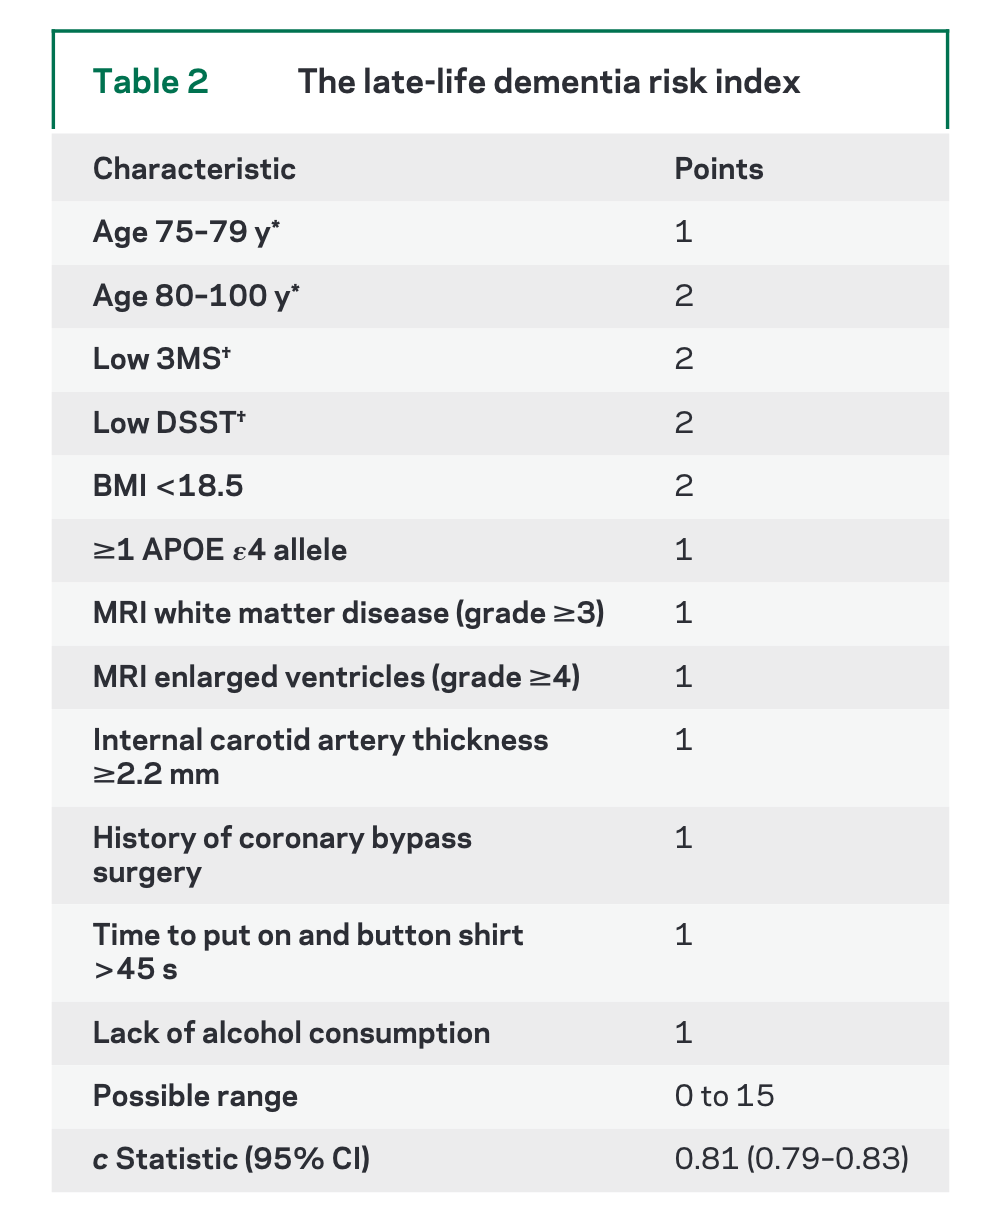
\includegraphics[width=7cm]{riskindex.png}
\caption{Late-life dementia risk index}
\label{risk}
\end{wrapfigure}
For every category, the variable which is most predictive of dementia is identified and then plugged into Eq.1, to calculate the logistic coefficients using multi-linear logistic regression. This approach considers the effect of all the variables together, which increases the chances of overfitting the model if there are too many predictors \cite{intro2013}. It is therefore important to make sure that only the most important predictors are included in the model. For this reason, the authors use a mixture of forward and backward sample selection procedure. The idea is quite straightforward. They started with no variables in the model, then add each predictors one by one and calculates the $p-$value of each variable in the model every time we add a new variable to make sure that all the variables maintain a $p-$ value below certain significance. If at any time, the $p-$ value of a variable rises above this threshold, that variable is removed from the model \cite{intro2013}. Once the model is finalized, the logistic coefficients are calculated.

\subsection{Developing the risk index}

The logistic coefficients (denoted by $\beta$) are a measure of how strong the relationship is between the predictor variables and the outcome of interest. Larger the value of $\beta$, stronger is the relationship and vice versa. If the coefficient is positive, it means that the predictor and the outcome is positively correlated. If the coefficient is negative, that means their relationship is negatively correlated. In this work, the authors assigned those predictors with magnitude of coefficients $>0.75$, 2 points and those with magnitude of logistic coefficients $\leq0.75$ 1 point, to create a table of late-life risk index (see Fig.\ref{risk} taken from \cite{barnes2009}).

\subsection{Accuracy of the model}

It is essential to quantify the accuracy of the model while applying to a new dataset. The predictive accuracy of the model is quantified using $c-$ statisitc. $c-$ statistics shows the extent of goodness-of-fit of the model \cite{cstat}. They plot the true positive rate against false positive rate (also called ROC curve) i.e, the risk score of a random person in the sample who has dementia vs risk score of random person who doesn't have dementia. Then the $c-$ statistic shows the probability of the former having a larger risk compared to the latter. We can see in Fig.\ref{risk} thet this probability is around 0.8. That implies a strong model. The authors also plotted the predicted percentage and the actual percentage of people who developed dementia against their risk index score calculated from Fig.\ref{risk}. It is very clear from Fig.\ref{plotrisk} (taken from \cite{barnes2009}) that, the model is quite accurate in risk prediction of dementia.  \\
\begin{wrapfigure}{r}{8cm}
\vspace{-10 mm}
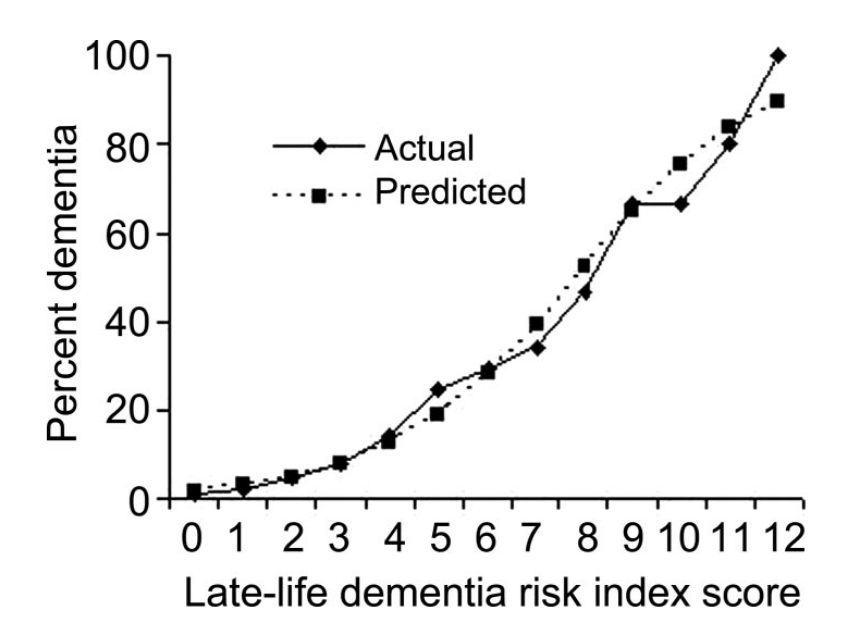
\includegraphics[width=8.2 cm]{riskplot.png}
\caption{Calibration of the late-life dementia risk index}
\label{plotrisk}
\end{wrapfigure}
In addition to this, it is important to evaluate the performance of the model when it comes to a new dataset. This process is called validation. Validation helps in estimating how good the trained model is with the new data. Low error on training data set doesn't guarantee low error on test data as it possible to get low errors on the former if the model is overfitting the data. Among several techniques to validate the model, the authors use $k-$ fold Cross Validation. The training dataset itself is randomly divided into $k$ groups of equal size. Then the first fold is considered as a test data set and the rest $k-1$ of them the training set. This process is repeated over every folds to generate $k$ estimates of test error \cite{intro2013}. An illustrative diagram taken from \cite{intro2013} is shown in Fig. \ref{cv}. The paper uses 10-fold Cross validation and $c-$ statistic to quantify the test error.


\begin{figure}[b!]
\centering
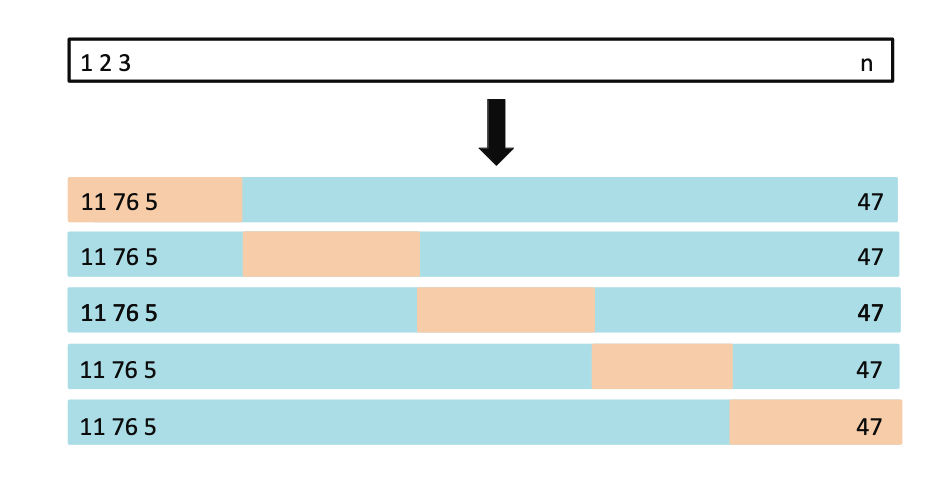
\includegraphics[width=13.2cm]{CV.png}
\caption{Diagram showing the process of $k-$ fold Cross Validation. Here the data is divided into 5 folds, so $k=5$ \cite{intro2013}. For the pupose of this study, the authors set $k=10$. }
\label{cv}
\end{figure}
\subsection{Discussion}

This study is focused on developing a dementia risk index for people who belong to the age group $\geq 65$. Though the initial sampling population consists of people who belong to the age range 65-100, the study found that the number of people who developed dementia who belonged to the age group of 65-74 is statistically insignificant. So the final risk index table consists of people who are older than 74. Among a huge range of predictors, using rigorous statistical analysis based on Logistic Regression, the authors narrowed down the most important predictors of dementia after correcting for the demographic factors and assigned them points based on the magnitude of logistic coefficients. With the risk index, one can calculate the risk index by summing up the points assigned to the predictor variables. 0 points corresponds to no risk of dementia and 15 points corresponds to a high risk domain. It is shown that the predictive model they developed shows high accuracy in categorizing individuals based on dementia risk through the results observed after 6 years during the follow up period. The 12 most important predictors chosen by statistics under which the model is based on, are among the most predictive factors for dementia shown by clinical research. \\

World Health Organization, in their website says that more than 55 million people worldwide has dementia. It is estimated that more than 6 million Americans have Alzheimer's disease which is a type of dementia. With this being the case, the study uses data of patients who belongs to four US counties with a sample size of 3,375. This is a quite small sample compared to the population who actually has dementia. Also may be it was better to randomly sample individuals across the whole nation instead of just four regions. In addition to this, the study even though it considers African Americans, the accuracy of this model when applied to people who are from other countries should be investigated.  Other than this, in my opinion, this study is quite comprehensive and exhaustive. The authors were very meticulous in selecting the most important predictor variables which helped them avoid overfitting their model. They eliminated the predictors at different stages of their analysis based on the $p-$ values and made sure the $p-$ values of variables in their model at every stage of their study were always below the chosen significance. They also quantified the accuracy of their model using $c-$ statistics and validated their model using the standard Cross validation approach. It might be interesting to apply the bayesian statistics to the same data and see what the risk index table looks like.


\section{Bayesian Approach to identifying potential risk factors for Dementia} 

In this section, we examine the study by Wen et al. (2016) \cite{Wen} where they try to identify potential risk factors for dementia using Bayesian statistics, based on nationwide longitudinal population-based data from Taiwan's National Health Insurance Research Database (NHIRD) \cite{taiwan}.

The study verifies 4 recognized risk factors for dementia:
\begin{itemize}
\item Severe head injury: Damage to the brain can lead to a decline in cognitive function which is associated with dementia.
\item Depression : Chronic depression can lead to changes in brain function.
\item Diabetes Mellitus: Low blood sugars are known to damage the the brain.
\item Vascular Diseases: Includes stroke, heart problems etc. This could cause reduced blood flow to the brain which can in turn damage it.
\end{itemize}

Additionally, the study also found hearing loss and senile cataracts as new potential risk factors for dementia. It also identifies $3$ demographic variables, namely, older age, female sex, and lower income as independent risk factors for dementia. \\

The use of Bayesian statistics in medical research has become increasingly popular in recent years, thanks to the growth of computational resources. Bayesian statistics, as described in the introduction, is a way to combine past (prior) and present (current study) evidence to make decisions about the future (posterior conclusions). By using Bayesian statistics, this study was able to identify new potential risk factors for dementia and help clinicians develop appropriate treatment strategies for patients at the early stages itself and prevent the worsening of this condition.

\subsection{Data and Study Design}
\begin{figure}[t]
\centering
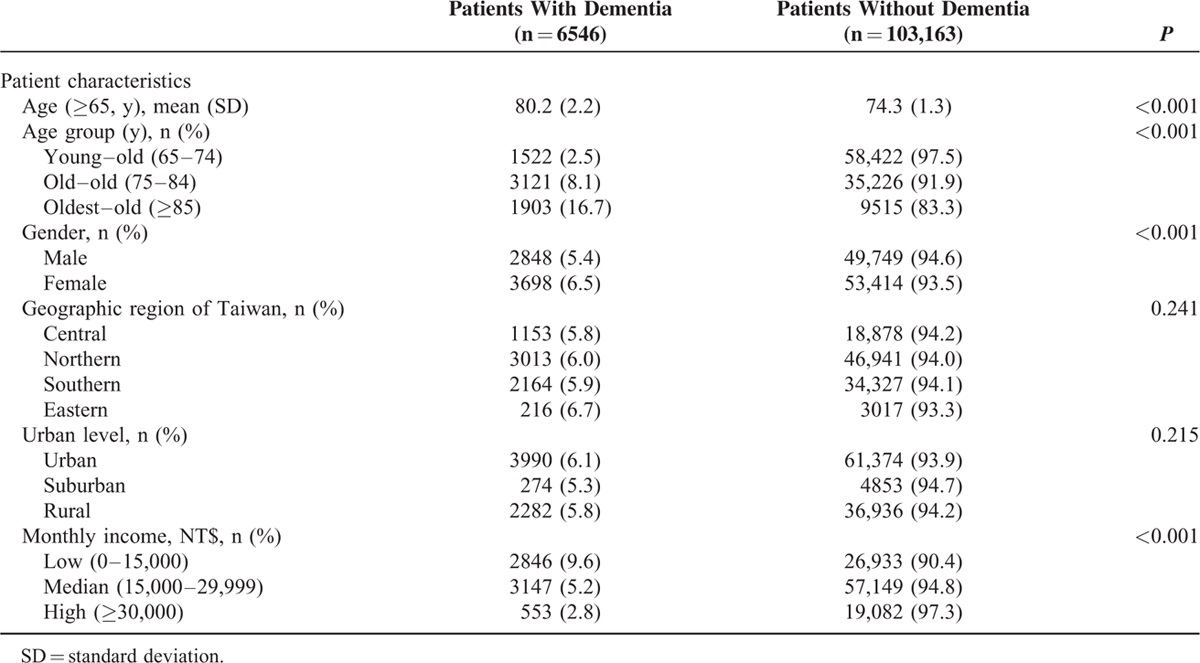
\includegraphics[width=1\linewidth]{bayesian_table1.jpeg}
\label{fig:bayesian_table1}
\caption{Demographics of the population}
\end{figure}

Of the 1,000,000 patients, the study includes 109,709 (11.0$\%$) patients aged $\geq 65$ years. A total of 6,546 (6.0$\%$) patients were diagnosed with dementia. Figure 5 shows the distribution of sociodemographic characteristics of the study population. Patients with dementia were significantly older than those without dementia (80.2 years vs 74.3 years). Moreover, the percentage of patients with dementia in the young–old (65–74 years), old–old (75–84 years), and oldest–old ($\geq$85 years) groups was significantly increased by 2.5$\%$, 8.1$\%$, and 16.7$\%$, respectively. The percentage of women with dementia was significantly higher than that of men with dementia (n = 3698, 6.5$\%$ vs 2848, 5.4$\%$). Furthermore, patients with high income had a significantly lower incidence of dementia than those with lower income (2.8$\%$, 5.2$\%$, and 9.6$\%$). \\

To make sure that the diagnosis of dementia was accurate, the authors only included patients who had been diagnosed with dementia at least once during a hospital stay, or had received a consistent diagnosis of dementia from their doctors during at least three outpatient visits. The first visit of the patients for the diagnosis of dementia is assigned as their index date. Then, the patients with dementia are assessed before or on their index date to ascertain their histories of Severe Head Injury, Depression, Diabetes Mellitus, Vascular Diseases, Senile Cataract, and Hearing Loss. The authors also looked at the medical records of patients who did not have dementia from 1995 to 2010 to see if they had any of the above risk factors, both when they were in the hospital and when they received medical care outside the hospital.

\subsection{Statistical Analysis}
The study attempts to learn about the unknown distribution from given data, to make some inferences about certain properties of the distribution, and then tries to determine the relative likelihood that each possible distribution is actually the correct one. \\

Let's say $\theta$ be the proportion of patients with dementia in the sample population. Then $ \mathbb{P}(\theta) \rightarrow$ Prior distribution of $\theta$. It is assumed to be a uniform distribution with $\mathbb{P}(\theta) = 1$ for $0 \le \theta \le 1$. Since the sample size is huge, the distribution of prior has a tiny impact on the posterior distribution. So it makes sense to choose such an ``informationless'' prior to reduce the computation cost. Now, let's define $x_i$, which is equal to $1$ if the $i_{th}$ person in the population has dementia, $0$ otherwise. Then, each of the $x_1, x_2, \dots, x_n$ follows a Bernoulli distribution with parameter $\theta$, where $n$ is the population size. So, the pdf of $x_i$ will be:
$$ \mathbb{P}(x_i | \theta) = \theta^{x_i}(1 - \theta)^{1-x_i} \text{, where } x_i \in \{0,1\}$$
Let's say $x = x_1, x_2, \dots, x_n$. Then, the joint probability distribution would be the product of $ \mathbb{P}(x_i | \theta)$ of all $x_i's$ which takes the form:
\begin{align*}
\mathbb{P}(x | \theta) = \theta^x(1-\theta)^{n - x} \tag*{} \\
\end{align*}

Note in the above equation, as we are only interested in the number of dementia cases not the number of possible combinations, there is no $^nC_x$ term. \\

Now, as the paper follows Bayesian approach, we need to estimate $\mathbb{P}(\theta | x)$.

\begin{align*}
\mathbb{P}(\theta | x) &= \mathbb{P}(x | \theta) \mathbb{P}(\theta) \text{      \tag*{[Bayes Theorem]}}\\
\implies \mathbb{P}(\theta | x) &= \theta^x(1-\theta)^{n - x} * 1 \text{ ; }\mathbb{P}(\theta) = 1 \\
\implies \mathbb{P}(\theta | x) &= \theta^x(1-\theta)^{n - x} \\
\end{align*}

As we can see $\mathbb{P}(\theta | x)$ came out to be Beta Distribution of the form $x^{\alpha-1}(1-x)^{\beta-1}$ with $\alpha = x + 1$ and $\beta = n - x + 1$. 


\subsubsection{Finding the Bayes Estimator}
We, here, explain and derive the Bayes estimator for the posterior probability distribution which the concerned study does not mention in detail.

The Bayes estimator is a function that specifies the estimated value of the parameter of interest for each possible set of values of observed data. In Bayesian inference, we start by assuming a prior distribution for the parameter of interest and then update our belief about it by incorporating the information from the data through the likelihood function. This results in the posterior distribution of the parameter given the data. The Bayes estimator is then defined as the function that minimizes the expected loss under this posterior distribution.
 
We will derive the Bayes estimator for the squared loss which is briefly mentioned in the study:
$$L(\theta, a) = (\theta - a)^2$$

where $\theta$ is the true value of the parameter and $a$ is the estimated value. \\

The Bayes estimator is then defined as the function $\delta(X)$ that minimizes the expected loss:
$$\delta(X) = \arg \min_a E_{\theta | X} [(a - \theta)^2]$$
where the expectation is taken with respect to the posterior distribution of $\theta$ given the observed data. \\

Expanding the squared term and rearranging, we get:

$$E_{\theta | X} [(a - \theta)^2] = E_{\theta | X} [(a - E_{\theta | X}[\theta] + E_{\theta | X}[\theta] - \theta)^2]$$

$$\implies E_{\theta | X} [(a - \theta)^2] = E_{\theta | X} [(a - E_{\theta | X}[\theta])^2] + E_{\theta | X} [(E_{\theta | X}[\theta] - \theta)^2] + 2E_{\theta | X}[(a - E_{\theta | X}[\theta])(E_{\theta | X}[\theta] - \theta)]$$ 

The first term is the variance of the estimator, which is independent of the choice of $a$. The second term is the mean squared error of the estimator, which measures the bias of the estimator. The third term is a cross-product term, which also depends on the choice of $a$.

To minimize the expected loss, we need to choose $a$ that minimizes the mean squared error term, which is equal to: $$E_{\theta | X} [(E_{\theta | X}[\theta] - a)^2]$$.

Taking the derivative of this expression with respect to $a$ and setting it to zero, we get:

$$2(E_{\theta | X}[\theta] - a) = 0$$
$$\implies a = E_{\theta | X}[\theta]$$

So, Bayes estimator in the case of the squared loss function comes out to be the posterior mean of the parameter, $$ \delta^*(x) = E_{\theta | x}[\theta] $$
$$ \delta^*(x) = \mathbb{E}(\theta | x)$$ \\
The mean of a beta distribution is $\frac{\alpha}{\alpha+\beta}$. So,
$$ \mathbb{E}(\theta | x) = \frac{x + 1}{n + 2}$$.
$$ \theta^* = \frac{x + 1}{n + 2}$$.

$\mathbb{E}(\theta | x)$ becomes the estimator of $\theta$ (we will denote it as $\theta^*$). \\

Finally, the study calculates the Odds-Ratio (OR) with respect to different factors. Odds-Ratio measures the odds of an outcome occurring in the exposed group compared to the odds of the same outcome occurring in the non-exposed group. It is the ratio of the posterior probability of $\theta$ to its complement. Odds-Ratio is used to measure association between two variables. An OR of 1 indicates no association between the exposure and outcome, while an OR greater than 1 indicates a positive association, meaning that the exposure is associated with an increased odds of the outcome.
$$ OR = \frac{\theta^*}{1 - \theta^*}$$

\begin{figure}
\centering
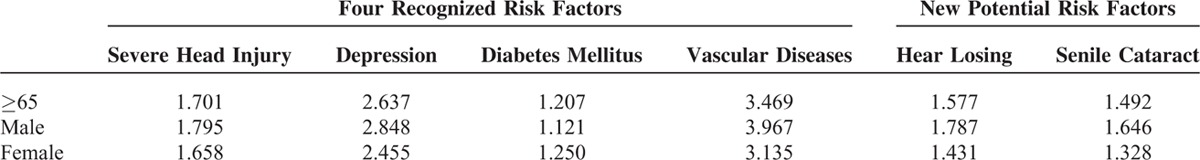
\includegraphics[width=1\linewidth]{figure6.jpeg}
\label{oddr}
\caption{Odd-Ratios for Dementia by Factors}
\end{figure}

\subsection{Results}

\begin{itemize}
\item Regarding the 4 recognized risk factors for dementia, Odd-Ratios in the older population with a history of severe head injury, depression, DM, and vascular diseases came out to be 1.701, 2.637, 1.207, and 3.469, respectively, as mentioned in Fig.6. Odd-Ratios for these risk factors were found to be higher in men with dementia than in women with dementia except for Diabetes Mellitus. 

\item Additionally,  Odd-Ratios of other potential risk factors, i.e., hearing loss (OR=1.577) and senile cataract (OR=1.492) were associated with an increased risk of dementia in the older population. In terms of sex-based differences, ORs of these risk factors were generally higher in men with dementia than in women with dementia.

\item The study found that the demographic factors such as older age, female sex, and lower income were also independent risk factors for dementia.

\item  The study identifies 2 new risk factors, namely, hearing loss and senile cataract. 
\end{itemize}


The study also highlighted that Taiwan has been an aging country since 1993, and the prevalence of dementia in the older population from 1995 to 2010 was approximately 6\%, similar to that in other developed countries. The study's results were consistent with previous studies, which identified older age, female sex, and lower socioeconomic status as risk factors for dementia in the East  \cite{Kalaria}. \\

The authors mention other studies that have found that certain medical conditions such as severe head injury, depression, diabetes, and vascular diseases, are associated with an increased risk of dementia. A review of 15 case-control studies \cite{Reitz} from 1991 to 2001 found that a history of head injury is a significant risk factor for Alzheimer's disease (AD) with a higher risk in men than women. However, the odds ratio (OR) in this study was lower than in the current study due to different criteria and disease diagnosis, but the difference in OR between sexes was similar. Another study based on the Taiwanese population found diabetes to be associated with an increased risk for AD. Furthermore, a systematic review \cite{Sawa} showed that a history of stroke doubles the risk of incident dementia in older adults. The ORs for the four recognized risk factors for dementia were higher in the current study than in other studies, possibly because the current study evaluated dementia while others evaluated AD which is a type of dementia.  \\

\subsection{Discussion}
As Taiwan's NHI program is a mandatory health insurance with affordable payments and services covering approximately 99\% of the Taiwanese population, the study did well in gathering a large data, ensuring that the data consists of a wide range of risk factors and a combination of risk factors also while keeping the biases to a minimum. \\

The paper also showcases the accuracy of its Bayesian approach, obtaining consistent results as that from other earlier studies implementing frequentist approaches. The paper is able to identify all the recognized risk factors obtained from other studies. While other risk factor assessment approaches use prior information by illustrating the levels or ranges of individual parameters in sensitivity analysis, the Bayesian method used domain knowledge to determine what is known about parameters and processes. However, the paper used data from the Taiwanese population, so its results can provide a good representation of risk factors for patients with dementia in ethnic Chinese populations, but cannot be generalized to other countries or ethnicities. \\

Moreover, as the data used does not include a lot of other information like  serum test results, body mass index, clinical severity of diseases, family history, and lifestyle of the patients, the study falls short of identifying further risk factors for Dementia. This study looked back at medical records to gather information on the patients, instead of following them over time just like the first study which uses a frequentist approach. Because of this, there is a possibility that the study may have been influenced by biases that can occur when looking back at past events. In addition to this, the authors hasn't quantified the predictive accuracy of the model they developed. 

\section{Bayesian or Frequentist?}
The two studies use different datasets of completely different populations and consider a lot of different factors. Therefore, we cannot directly compare the two studies, and decide which one turned out better. We, however, still try to compare some of the findings and assess the similarities and differences. We try to compare the results of the two studies by comparing the quantities that came out to be strong factors/predictors for Dementia. Both papers are able to identify Age and Gender as important factors. The frequentist approach also gets cognitive ability and alcohol consumption as important factors, but we cannot compare this result with the bayesian approach as it did not take these quantities into consideration. The two paper diverges in finding the significance of pre-existing medical conditions. While the medical conditions did not come out to be strong predictors in the frequentist approach, in Bayesian approach, they (Severe Head Injury, Diabetes etc) are the most significant factors. This could be because the bayesian paper considers only a few risk factors to begin with whereas the paper which uses the frequentist approach considers a large number of factors, then based on their statistical significance eliminated the least important factors. So it is possible that the 
pre-existing medical conditions emerged to be on the top in the absence of other significant risk factors. It would be interesting to see if applying the same methodology as in the bayesian paper to a wide range of predictors change the outcome. It should however be noted that the history of having a bypass surgery is a risk factor (which is a pre-exisiting medical condition) is among the risk factors used to calculate the dementia risk index in the frequentist paper, but it is assigned a point score of 1 (i.e., not among the most important factors). Also, the bayesian analysis is based on a nation-wide survey and has a very large sample size as opposed to the frequentist analysis which is based on a localised survey and consists of data of around $\sim$ 3000 individuals. \\

In conclusion, both approaches found results consistent with existing literature making it impossible to favor one study over the other. One approach is not clearly better than the other, and choosing one over the other depends on the availability of the data and individual choice. The frequentist approach uses a small data of regional population of the USA, where Bayesian approach leverages a large dataset of the Taiwanese population. Therefore, we could not have a direct fair comparison between the two, however, we still compared the significant factors. We found that the two are able to identify a lot of similar factors, already known to be significant in the existing literature. As a future step, in order to have a fair comparison we could apply both approaches to the same data. 


\begin{thebibliography}{}
\bibitem {chen2018} Chen, Yen-Chi., ``Review on Statistical Inference'',STAT 516, Stochastic Modeling of Scientific Data, University of Washington, 2018. 
\bibitem {mary} Parker, Mary., http://www.austincc.edu/mparker/stat/nov04/
\bibitem {dem} https://www.alz.org/alzheimers-dementia/what-is-dementia
\bibitem{Croat}  BK. Bayes or not Bayes, is this the question? Croat Med J. 2019 Feb 28;60(1):50-52. doi: 10.3325/cmj.2019.60.50. PMID: 30825279; PMCID: PMC6406060.
\bibitem{abc} https://towardsdatascience.com/statistics-are-you-bayesian-or-frequentist-4943f953f21b
\bibitem{barnes2009} Barnes DE, Covinsky KE, Whitmer RA, Kuller LH, et al., Predicting risk of dementia in older adults: The late-life dementia risk index. Neurology. 2009, 173-9.
\bibitem{Wen} Wen YH, Wu SS, Lin CR et al., A Bayesian Approach to Identifying New Risk Factors for Dementia: A Nationwide Population-Based Study, Medicine (Baltimore), 2016
\bibitem{intro2013} James, G., Witten, D., Hastie, T., \& Tibshirani, R. (2013). An introduction to statistical learning: with applications in R. Springer.
\bibitem{sigmoid} https://www.datacamp.com/tutorial/logistic-regression-R
\bibitem {Kuller2003} Kuller LH, Lopez OL, Newman A, et al., Risk factors for dementia in the cardiovascular health cognition study. Neuroepidemiology 2003, 13–22
\bibitem {Lopez2003} Lopez OL, Kuller LH, Fitzpatrick A, et al., Evaluation of dementia in the cardiovascular health cognition study. Neuroepidemiology 2003, 1–12.
\bibitem{cholest} https://www.hopkinsmedicine.org/health/treatment-tests-and-therapies/lipid-panel
\bibitem {cart1} Loh, WeiYin. “Classification and regression tree methods.” Encyclopedia of statistics in quality and reliability, 2008.
\bibitem {cart2} Morgan, Jake., Classification and Regression Tree Analysis, 2014. https://www.bu.edu/sph/files/2014/05/MorganCART.pdf
\bibitem {cart3} Lemon SC, Roy J, Clark MA, et al., Classification and regression tree analysis in public health: methodological review and comparison with logistic regression., Ann Behav Med. 2003, 172-81. 
\bibitem {cart4} Van Putten W. CART: Stata module to perform Classification and Regression Tree analysis. In: Statistical Software Components S456776: Boston College Department of Economics; 2006.
\bibitem{chisq} Beyer, Alisa., Introduction to Statistics for Psychology, 2021.
\bibitem{cstat} Glen, Stephanie., ``C-Statistic: Definition, Examples, Weighting and Significance'' From StatisticsHowTo.com. https://www.statisticshowto.com/c-statistic/
\bibitem{taiwan}  Cheng TM. Okma KGH, Crivelli L. Taiwan's National Health Insurance System: High Value for the Dollar. Six Countries, Six Reform Models: The Health Reform Experience of Israel, the Netherlands, New Zealand, Singapore, Switzerland and Taiwan.. New Jersey: World Scientific, 2009. 71–204.
\bibitem{Kalaria} Kalaria, Raj N., Gladys E. Maestre, Raul Arizaga et al., "Alzheimer's disease and vascular dementia in developing countries: prevalence, management, and risk factors." The Lancet Neurology 7, 2008, 812-826.
\bibitem{Sawa} Sawa GM, Stephan BC. Alzheimer's Society Vascular Dementia Systematic Review Group. Epidemiological studies of the effect of stroke on incident dementia: a systematic review. Stroke, 2010.
\bibitem{Reitz} Reitz C, Mayeux R. Alzheimer disease: epidemiology, diagnostic criteria, risk factors and biomarker. Biochem Pharmacol, 2014, 640–651.

\end{thebibliography}




\end{document}
